\documentclass{beamer}
\mode<presentation>
\usepackage{amsmath,amssymb,mathtools}
\usepackage{textcomp}
\usepackage{gensymb}
\usepackage{adjustbox}
\usepackage{subcaption}
\usepackage{enumitem}
\usepackage{multicol}
\usepackage{listings}
\usepackage{url}
\usepackage{graphicx} % <-- needed for images
\def\UrlBreaks{\do\/\do-}

\usetheme{Boadilla}
\usecolortheme{lily}
\setbeamertemplate{footline}{
  \leavevmode%
  \hbox{%
  \begin{beamercolorbox}[wd=\paperwidth,ht=2ex,dp=1ex,right]{author in head/foot}%
    \insertframenumber{} / \inserttotalframenumber\hspace*{2ex}
  \end{beamercolorbox}}%
  \vskip0pt%
}
\setbeamertemplate{navigation symbols}{}

\lstset{
  frame=single,
  breaklines=true,
  columns=fullflexible,
  basicstyle=\ttfamily\tiny   % tiny font so code fits
}

\numberwithin{equation}{section}

% ---- your macros ----
\providecommand{\nCr}[2]{\,^{#1}C_{#2}}
\providecommand{\nPr}[2]{\,^{#1}P_{#2}}
\providecommand{\mbf}{\mathbf}
\providecommand{\pr}[1]{\ensuremath{\Pr\left(#1\right)}}
\providecommand{\qfunc}[1]{\ensuremath{Q\left(#1\right)}}
\providecommand{\sbrak}[1]{\ensuremath{{}\left[#1\right]}}
\providecommand{\lsbrak}[1]{\ensuremath{{}\left[#1\right.}}
\providecommand{\rsbrak}[1]{\ensuremath{\left.#1\right]}}
\providecommand{\brak}[1]{\ensuremath{\left(#1\right)}}
\providecommand{\lbrak}[1]{\ensuremath{\left(#1\right.}}
\providecommand{\rbrak}[1]{\ensuremath{\left.#1\right)}}
\providecommand{\cbrak}[1]{\ensuremath{\left\{#1\right\}}}
\providecommand{\lcbrak}[1]{\ensuremath{\left\{#1\right.}}
\providecommand{\rcbrak}[1]{\ensuremath{\left.#1\right\}}}
\theoremstyle{remark}
\newtheorem{rem}{Remark}
\newcommand{\sgn}{\mathop{\mathrm{sgn}}}
\providecommand{\abs}[1]{\left\vert#1\right\vert}
\providecommand{\res}[1]{\Res\displaylimits_{#1}}
\providecommand{\norm}[1]{\lVert#1\rVert}
\providecommand{\mtx}[1]{\mathbf{#1}}
\providecommand{\mean}[1]{E\left[ #1 \right]}
\providecommand{\fourier}{\overset{\mathcal{F}}{ \rightleftharpoons}}
\providecommand{\system}{\overset{\mathcal{H}}{ \longleftrightarrow}}
\providecommand{\dec}[2]{\ensuremath{\overset{#1}{\underset{#2}{\gtrless}}}}
\newcommand{\myvec}[1]{\ensuremath{\begin{pmatrix}#1\end{pmatrix}}}
\let\vec\mathbf

\title{MatGeo Presentation - Problem 5.5.16}
\author{EE25BTECH11064 - Yojit Manral}
\date{}

\begin{document}

\frame{\titlepage}
\begin{frame}{Question}
\begin{align}
    \vec{A} = \myvec{2&-3&5\\3&-2&-4\\1&1&-2}
\end{align}
Find $\vec{A}^{-1}$. Use it to solve the given system of equations
\begin{align}
2x - 3y + 5z = 11 \\
3x - 2y - 4z = -5 \\
x + y - 2z = -3
\end{align}
\end{frame}

\begin{frame}{Solution}
$\rightarrow$ Using the properties of inverses
\begin{align}
    \vec{A} \vec{A}^{-1} &= \vec{I}_{3\times3} \\
    \myvec{2&-3&5\\3&-2&-4\\1&1&-2}\vec{A}^{-1} &= \myvec{1&0&0\\0&1&0\\0&0&1}
\end{align}
$\rightarrow$ Now, using augmented matrix
\begin{align}
\left(\begin{array}{ccc|ccc} 2&-3&5&1&0&0\\3&-2&-4&0&1&0\\1&1&-2&0&0&1 \end{array}\right)
\xrightarrow{R_1 \leftrightarrow (1/2)R_1} \left(\begin{array}{ccc|ccc} 1&-3/2&5/2&1/2&0&0\\3&-2&-4&0&1&0\\1&1&-2&0&0&1 \end{array}\right) \\
\xrightarrow{R_2 \leftrightarrow R_2 - 3R_1} \left(\begin{array}{ccc|ccc} 1&-3/2&5/2&1/2&0&0\\0&5/2&-23/2&-3/2&1&0\\1&1&-2&0&0&1 \end{array}\right)
\end{align}
\end{frame}

\begin{frame}{Solution}
\begin{align}
\xrightarrow{R_3 \leftrightarrow R_3 - R_1} \left(\begin{array}{ccc|ccc} 1&-3/2&5/2&1/2&0&0\\0&5/2&-23/2&-3/2&1&0\\0&5/2&-9/2&-1/2&0&1 \end{array}\right) \\
\xrightarrow{R_3 \leftrightarrow R_3 - R_2} \left(\begin{array}{ccc|ccc} 1&-3/2&5/2&1/2&0&0\\0&5/2&-23/2&-3/2&1&0\\0&0&7&1&-1&1 \end{array}\right) \\
\xrightarrow{R_2 \leftrightarrow (2/5)R_2} \left(\begin{array}{ccc|ccc} 1&-3/2&5/2&1/2&0&0\\0&1&-23/5&-3/5&2/5&0\\0&0&7&1&-1&1 \end{array}\right) \\
\xrightarrow{R_3 \leftrightarrow (1/7)R_3} \left(\begin{array}{ccc|ccc} 1&-3/2&5/2&1/2&0&0\\0&1&-23/5&-3/5&2/5&0\\0&0&1&1/7&-1/7&1/7 \end{array}\right)
\end{align}
\end{frame}

\begin{frame}{Solution}
\begin{align}
\xrightarrow{R_1 \leftrightarrow R_1 + (3/2)R_2} \left(\begin{array}{ccc|ccc} 1&0&-22/5&-2/5&3/5&0\\0&1&-23/5&-3/5&2/5&0\\0&0&1&1/7&-1/7&1/7 \end{array}\right) \\
\xrightarrow{R_2 \leftrightarrow R_2 + (23/5)R_3} \left(\begin{array}{ccc|ccc} 1&0&-22/5&-2/5&3/5&0\\0&1&0&2/35&-9/35&23/35\\0&0&1&1/7&-1/7&1/7 \end{array}\right) \\
\xrightarrow{R_1 \leftrightarrow R_1 + (22/5)R_3} \left(\begin{array}{ccc|ccc} 1&0&0&8/35&-1/35&22/35\\0&1&0&2/35&-9/35&23/35\\0&0&1&1/7&-1/7&1/7 \end{array}\right) \\
\implies \vec{A}^{-1} = \frac{1}{35}\myvec{8&-1&22\\2&-9&23\\5&-5&5}
\end{align}
\end{frame}

\begin{frame}{Solution}
$\rightarrow$ From (2), (3) and (4), we get
\begin{align}
    \myvec{2&-3&5\\3&-2&-4\\1&1&-2} \myvec{x\\y\\z} &= \myvec{11\\-5\\-3} \\
    \vec{A}\hspace{1.5cm}\vec{x}\hspace{0.35cm} & \hspace{1cm}\vec{B} \notag
\end{align}
$\rightarrow$ So, we compute
\begin{align}
    \vec{x} &= \vec{A}^{-1} \vec{B} \\
    \vec{x} &= \frac{1}{35}\myvec{8&-1&22\\2&-9&23\\5&-5&5}\myvec{11\\-5\\-3} \\
    \vec{x} &= \myvec{27/35\\-2/35\\13/7}
\end{align}
\end{frame}

\begin{frame}{Solution}
\begin{figure}[h!]
   \centering
   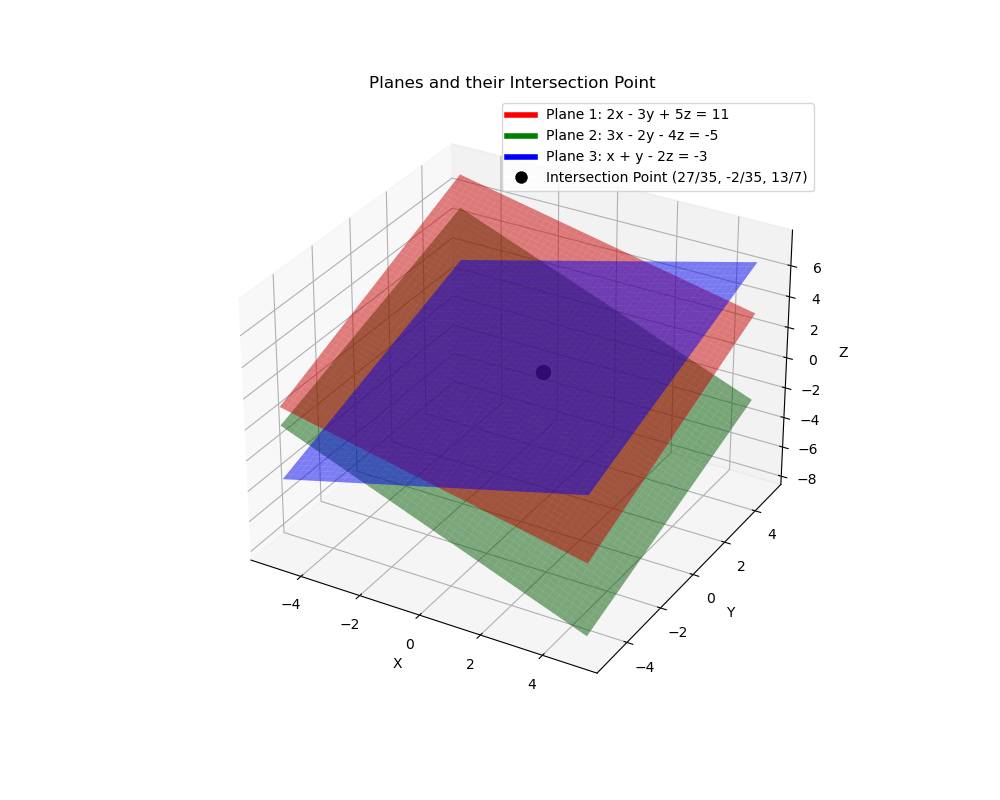
\includegraphics[width=0.8\linewidth]{figs/01.png}
   \caption{Plot of system of equations}
   \label{Plot_1}
\end{figure}
\end{frame}
 % --------- CODE APPENDIX ---------
\section*{Appendix: Code}

% C program
\begin{frame}[fragile]{File: points.c}
\begin{lstlisting}[language=C]
#include <stdio.h>

int main() {
  FILE *fp;

  // -------------------
  // Question 5.5.16
  // -------------------


  fp = fopen("points.dat", "w");
  fprintf(fp, "%d,%d,%d\n", 2, -3, 5); // A
  fprintf(fp, "%d,%d,%d\n", 3, -2, -4); // B
  fprintf(fp, "%d,%d,%d\n", 1, 1, -2); // C
  fprintf(fp, "%f,%f,%f\n", 27/35, -2/35, 13/7); // P
  fclose(fp);
  return 0;
}
\end{lstlisting}
\end{frame}

% Python calling C
\begin{frame}[fragile]{File: call\_c.py}
\begin{lstlisting}[language=Python]
import subprocess

# Compile the C program
subprocess.run(["gcc", "points.c", "-o", "points"])

# Run the compiled C program
result = subprocess.run(["./points"], capture_output=True, text=True)

# Print the output from the C program
print(result.stdout)
\end{lstlisting}
\end{frame}

% Python plotting
\begin{frame}[fragile]{File: plot.py}
\begin{lstlisting}[language=Python]
import numpy as np
import matplotlib.pyplot as plt

# Plane functions:
def plane1(x, y):
    return (11 - 2*x + 3*y) / 5

def plane2(x, y):
    return -(3*x - 2*y + 5) / 4

def plane3(x, y):
    return (x + y + 3) / 2

# Create grid
x = np.linspace(-5, 5, 50)
y = np.linspace(-5, 5, 50)
X, Y = np.meshgrid(x, y)

Z1 = plane1(X, Y)
Z2 = plane2(X, Y)
Z3 = plane3(X, Y)

# Intersection point
x_int = 27/35
y_int = -2/35
z_int = 13/7

# Plotting
fig = plt.figure(figsize=(10, 8))
ax = fig.add_subplot(111, projection='3d')
\end{lstlisting}
\end{frame}

% Python plotting
\begin{frame}[fragile]{File: plot.py}
\begin{lstlisting}[language=Python]
ax.plot_surface(X, Y, Z1, alpha=0.5, color='red', label='2x - 3y + 5z = 11')
ax.plot_surface(X, Y, Z2, alpha=0.5, color='green', label='3x - 2y - 4z = -5')
ax.plot_surface(X, Y, Z3, alpha=0.5, color='blue', label='x + y - 2z = -3')

# Plot the intersection point
ax.scatter(x_int, y_int, z_int, color='black', s=100, label='Intersection Point')

# Labels and title
ax.set_xlabel('X')
ax.set_ylabel('Y')
ax.set_zlabel('Z')
ax.set_title('Planes and their Intersection Point')

# Legend (manual, since plot_surface doesn't handle labels well)
from matplotlib.lines import Line2D
custom_lines = [Line2D([0], [0], color='red', lw=4),
                Line2D([0], [0], color='green', lw=4),
                Line2D([0], [0], color='blue', lw=4),
                Line2D([0], [0], marker='o', color='w', markerfacecolor='black', markersize=10)]
ax.legend(custom_lines, ['Plane 1: 2x - 3y + 5z = 11', 
                        'Plane 2: 3x - 2y - 4z = -5', 
                        'Plane 3: x + y - 2z = -3', 
                        'Intersection Point (27/35, -2/35, 13/7)'])

plt.show()

\end{lstlisting}
\end{frame}

\end{document}
